\documentclass[10pt,a4paper]{article}
\usepackage[utf8]{inputenc}
\usepackage{amsmath}
\usepackage{amsfonts}
\usepackage{amssymb}
\usepackage{graphicx}
\usepackage{enumerate}
\begin{document}

\section{Set Theory}

To demystify mathematics consider
\begin{enumerate}[(i)]
\item What is a theorem?
\item What is a proof?
\end{enumerate}
What if we don't know the answer?

To begin we need
\begin{enumerate}[(a)]
\item an example(s)
\item a nearly related concept
\end{enumerate}


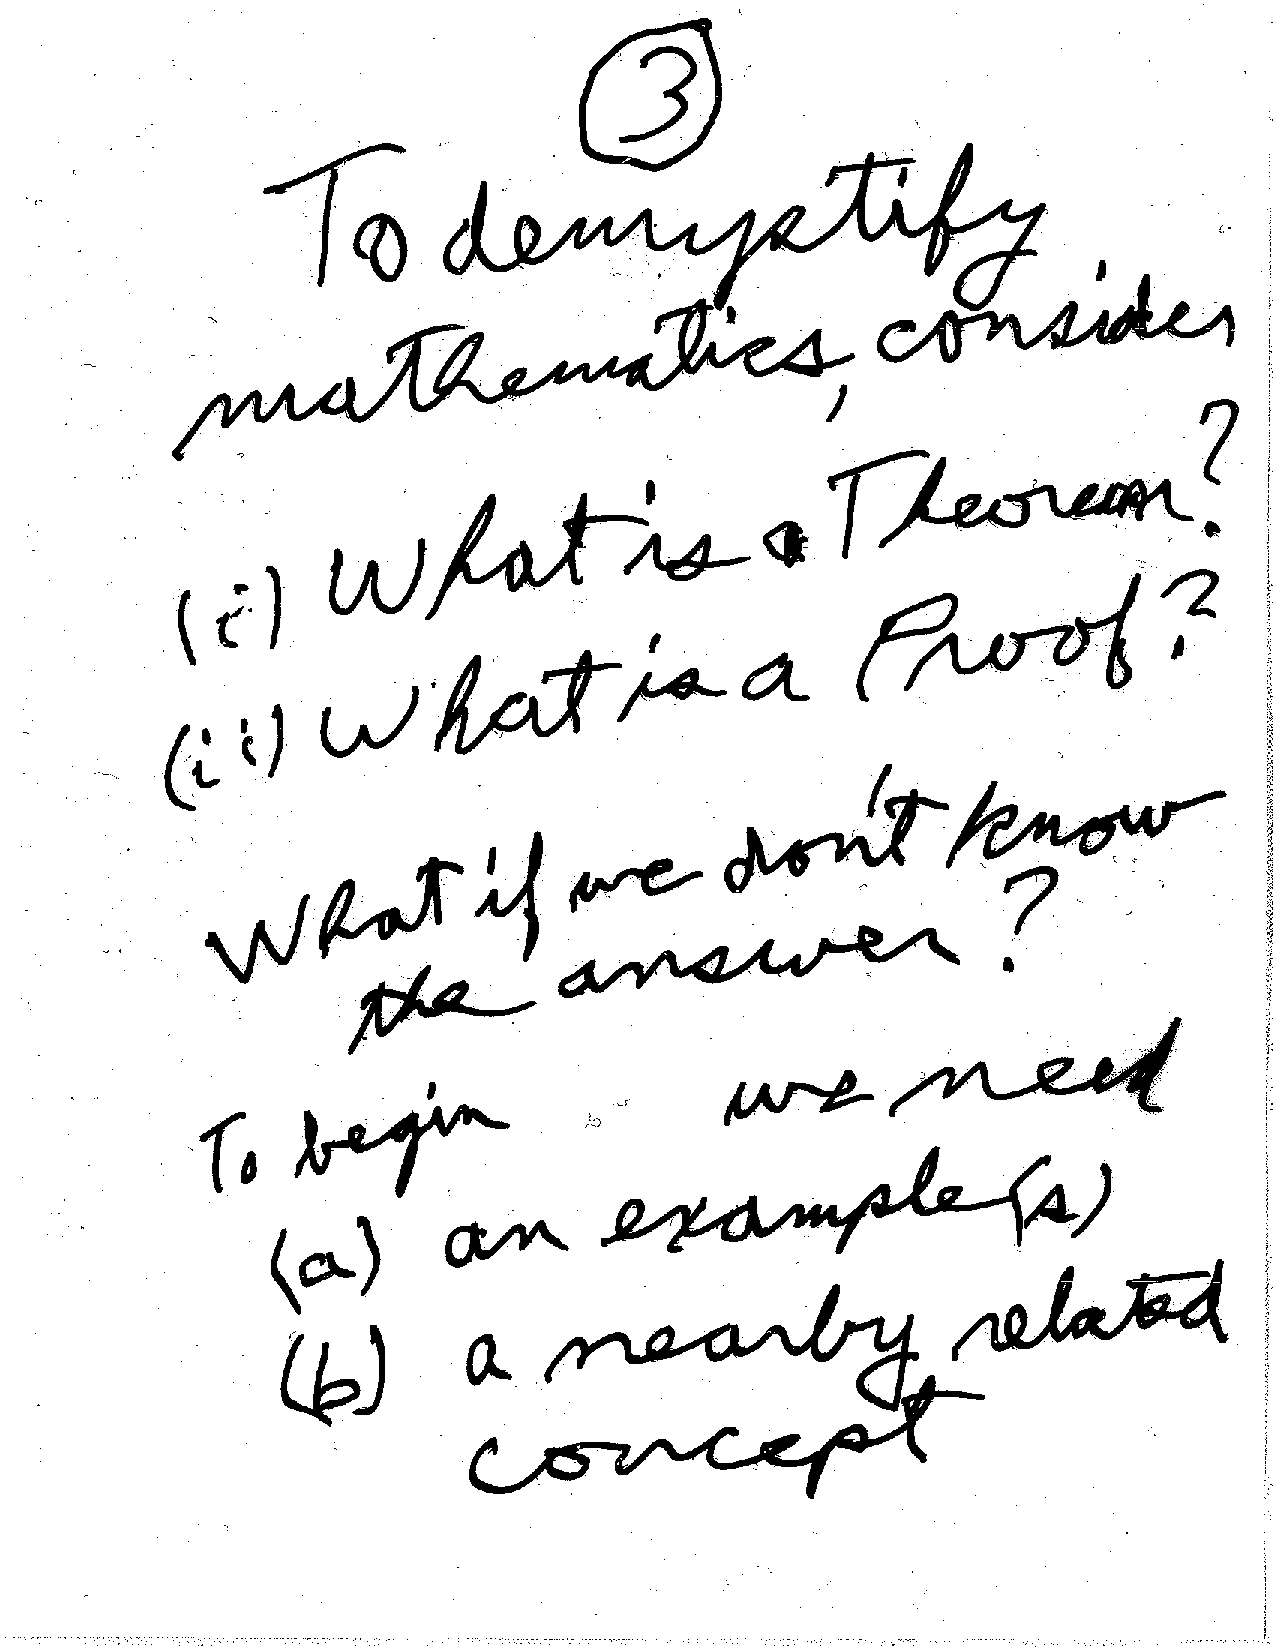
\includegraphics[scale=.5]{Pages/ST_3}

\newpage

Related Concept: Greek Syllogism

\underline{example:}
\begin{enumerate}
\item All men are mortal.
\item Socrates is a man.
\item Therefore, Socrates must die. 
\end{enumerate}

To analyze, recast in set theoretic terms via Venn Diagram.

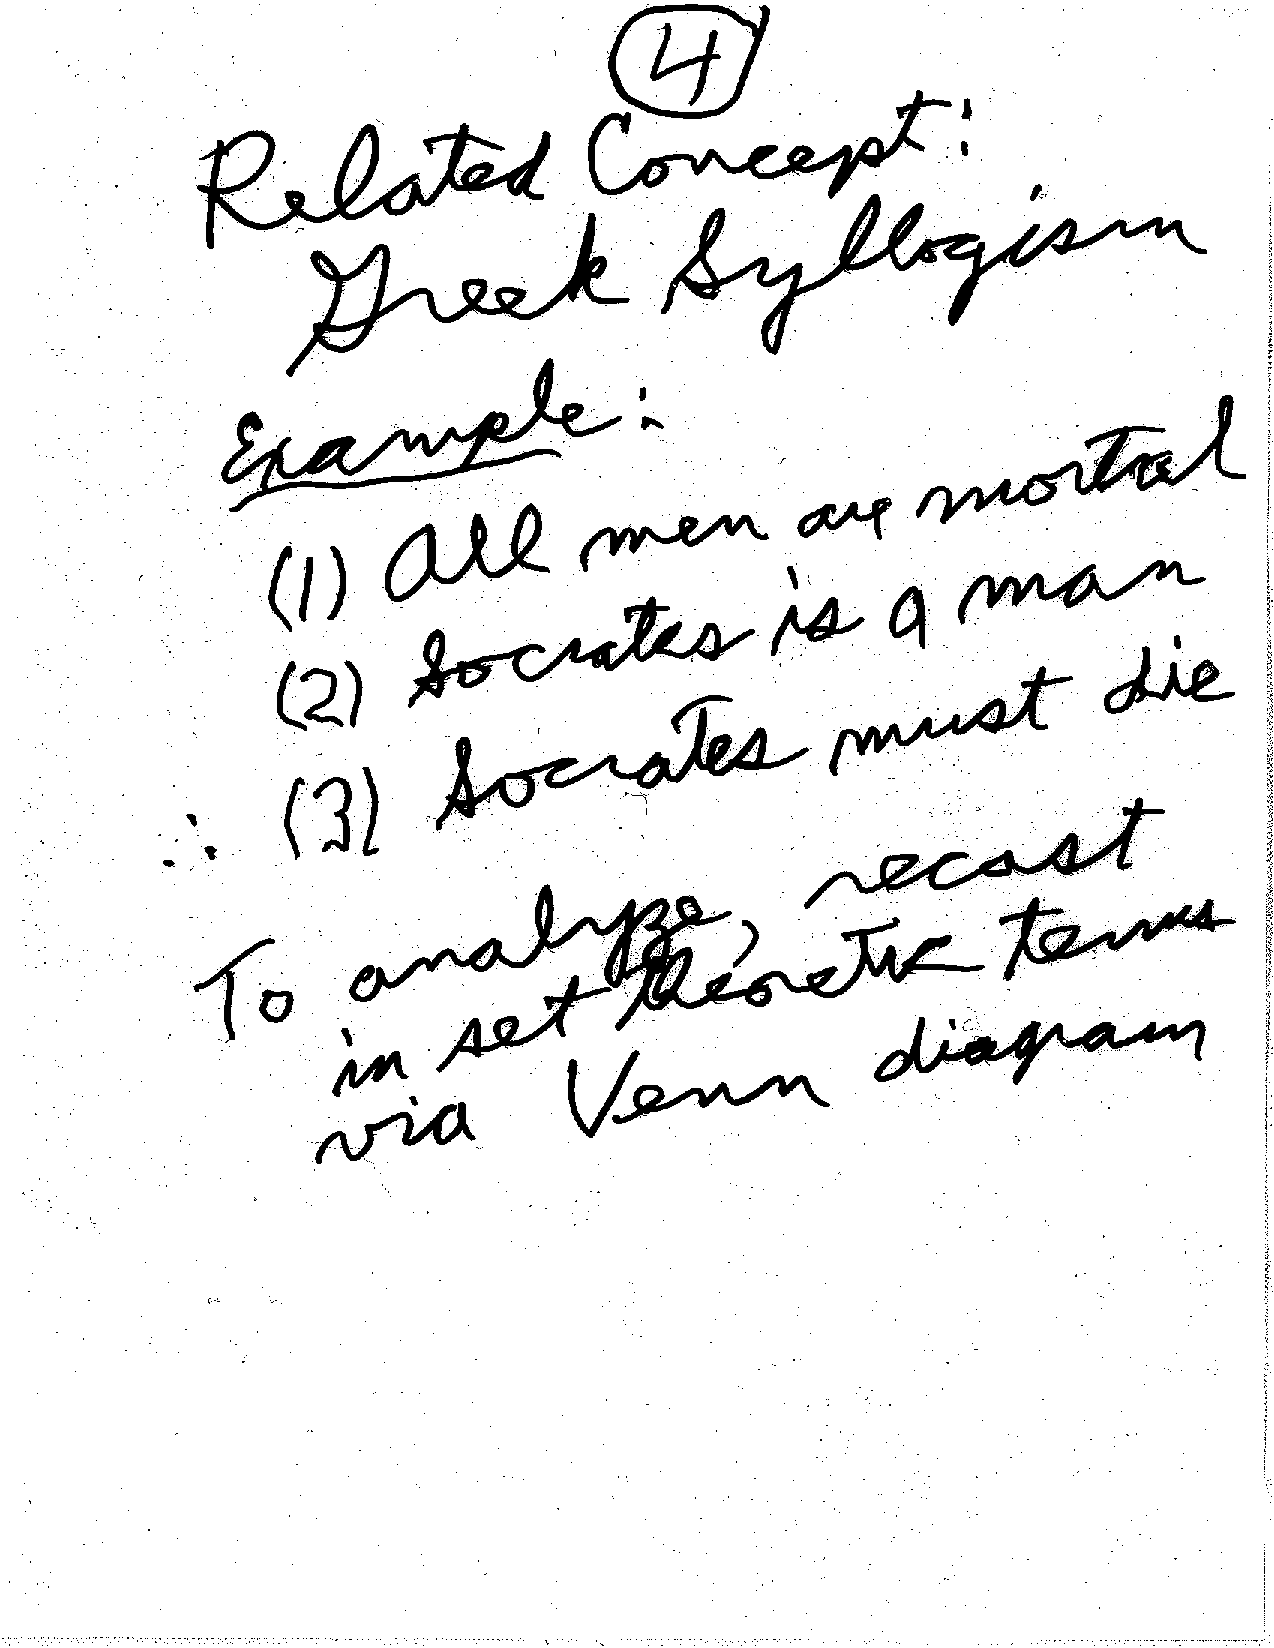
\includegraphics[scale=.5]{Pages/ST_4}

\newpage

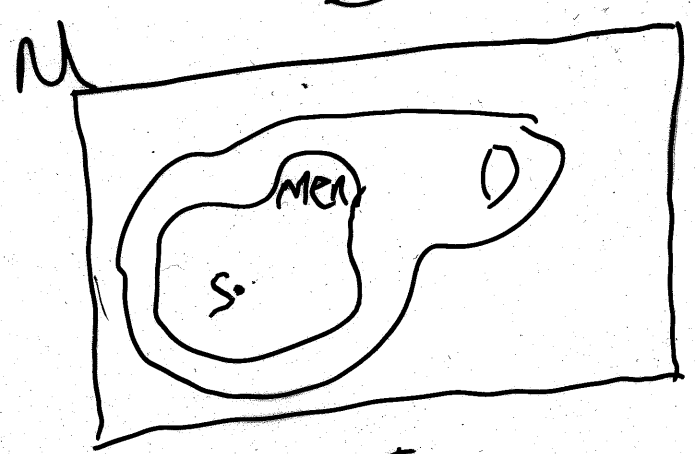
\includegraphics[scale=.2]{Pages/ST_5_im1}

$S$: Socrates\\
$M$: Set of Men\\
$D$: Things that will die\\
$\mathcal{U}$: Things on Earth

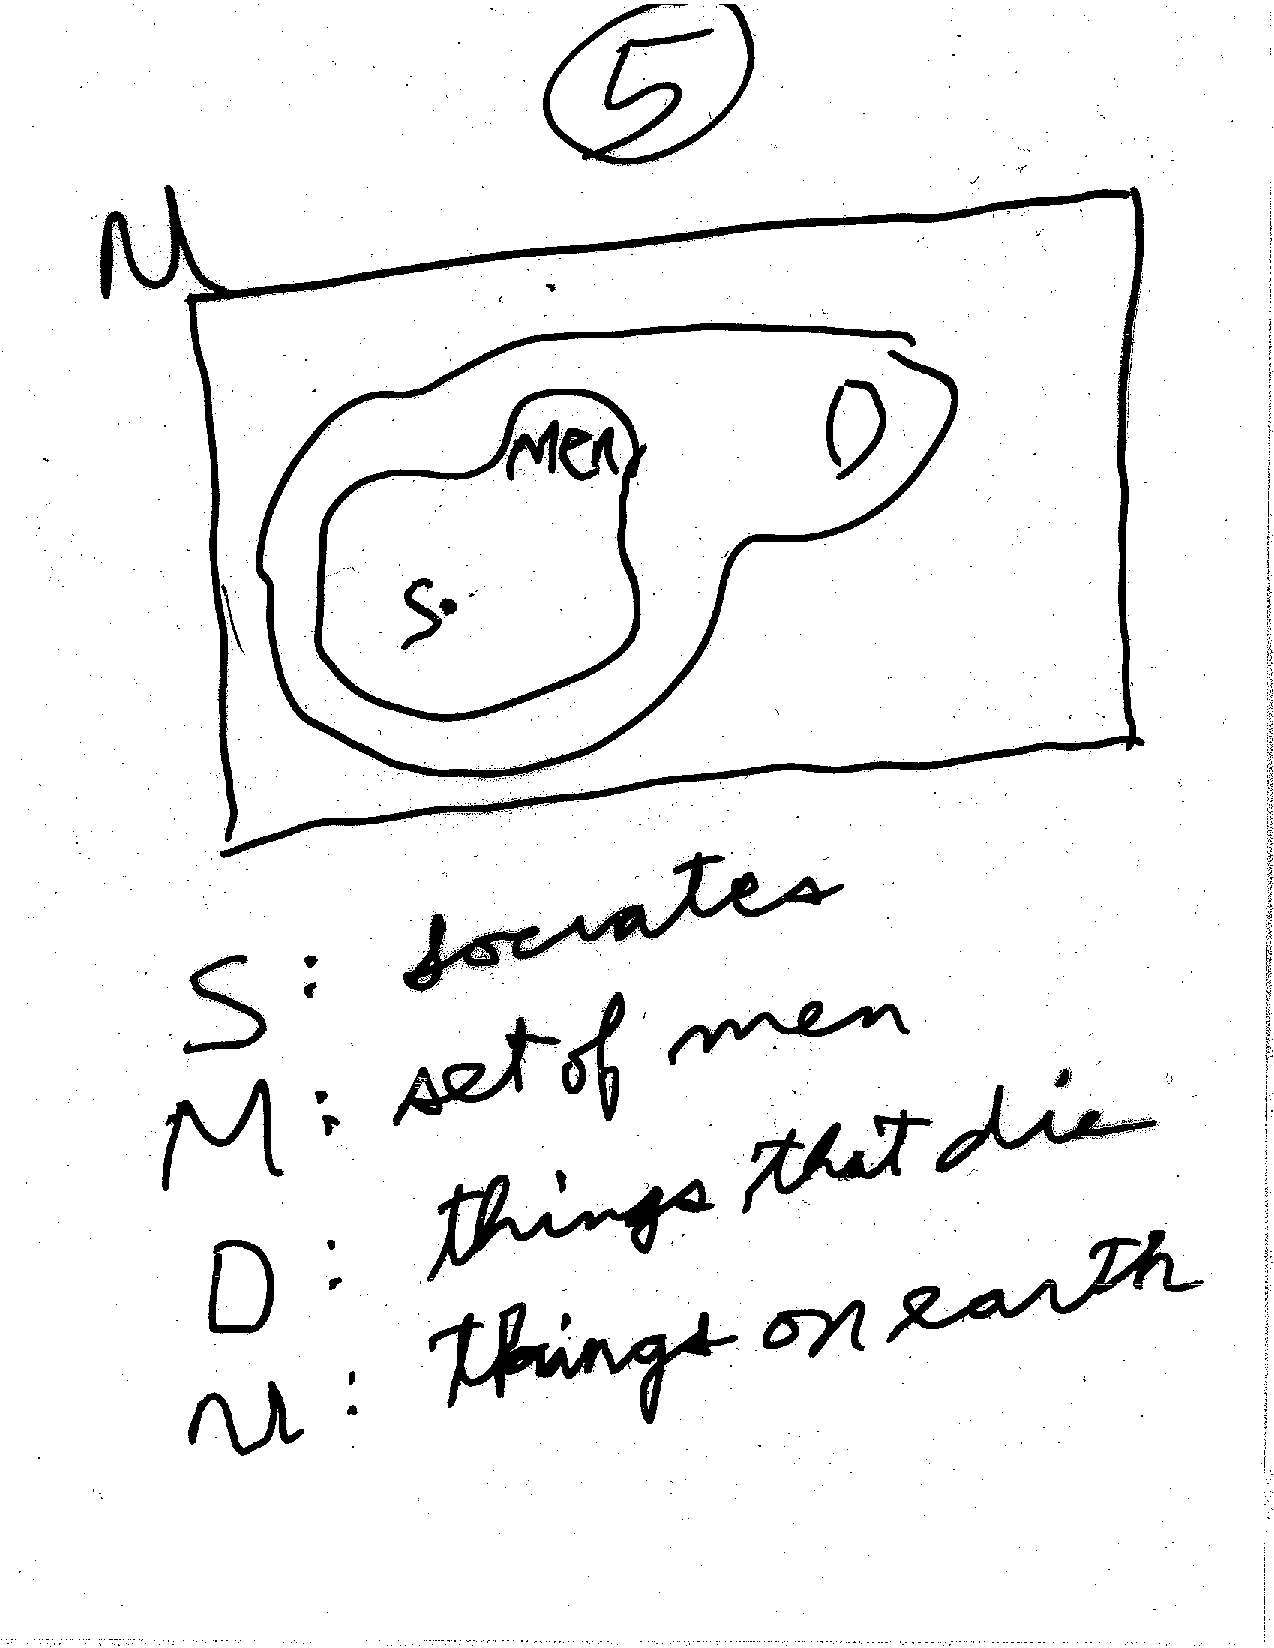
\includegraphics[scale=.5]{Pages/ST_5} 



%Zack: Pages 6,7,8,19,20

%Jack: 21, 9, 10, 11

%Koka: Pages 13, 13A, 22 ,22A, 22B


\section{Generate $\mathbb{N}$}


%Ruth: Pages L4A-L4G




\section{From $\mathbb{Z}$ to $\mathbb{R}$ via ordering}
%Jazz: ZR1-ZR5

%Kyler: ZR6 - ZR10

%Preethika: ZR11-ZR14


\section{Sequence and Limits}

%Aaron: First 2 pages and 48-50

%Hamza: 51-52B
{Theorem Suppose $a_n \rightarrow a$ and $b_n \rightarrow b$. Then $a_n + b_n \rightarrow a + b$ (and $ \lambda a_n \rightarrow	\lambda a$)and $a_n b_n \rightarrow a * b$}\newline

{Theorem if $a_n \rightarrow a \neq 0$, then $\frac{1}{a_n} \rightarrow \frac{1}{a}$}\newline

{corollary if $a_n \rightarrow a$ and $b_n \rightarrow b \neq 0$ then $\frac{a_n}{b_n} \rightarrow \frac{a}{b}$} \newline

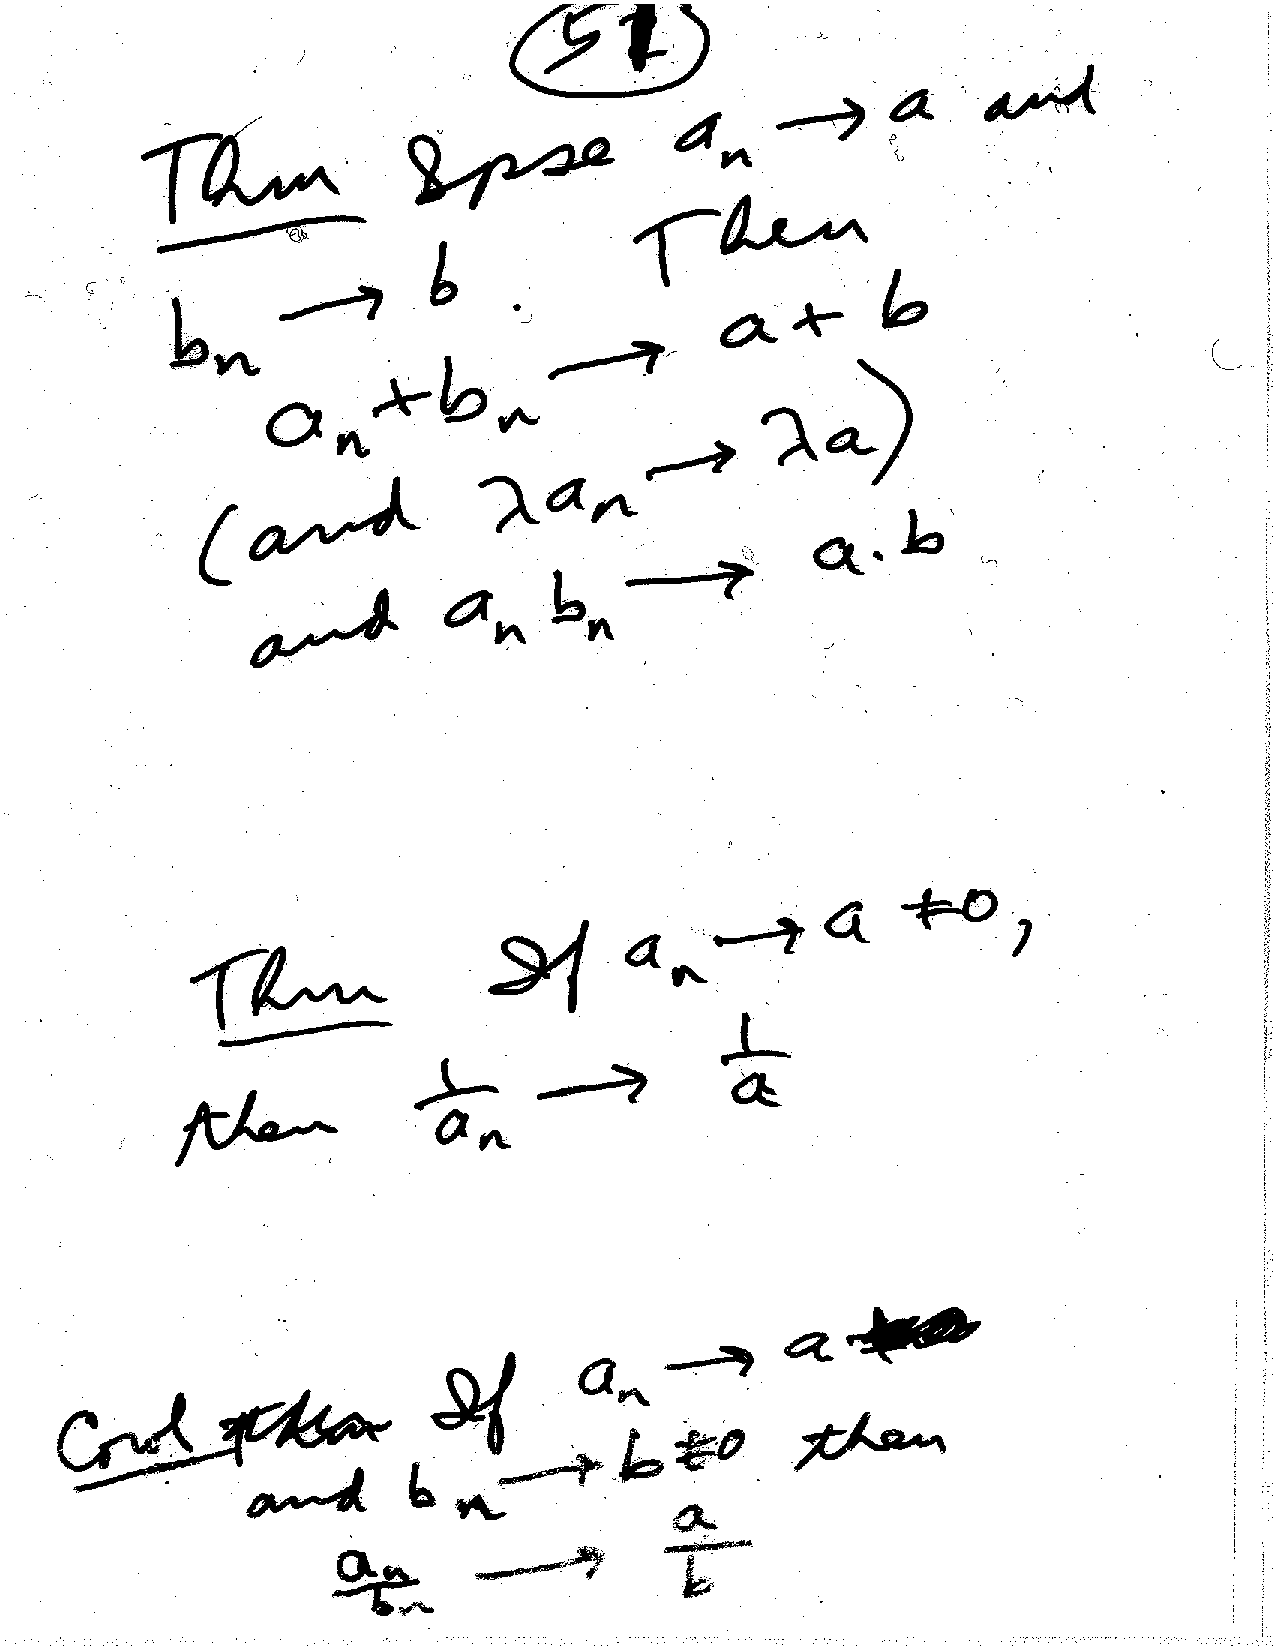
\includegraphics[scale=.5]{Pages/SL_7} 

\newpage
\underline{A method of proving corner:}\newline
\underline{monotone sequences} \newline
Lat $\{a_n\}$ be a sequence of reals. We say $\{a_n\}$ is \underline{monotonic} if either $a_1 \leq a_2 ... \leq a_a \leq ...$
or else $a_1 \geq  a_2 ... \geq a_a \geq ...$ 
In the first case $\{a_n\}$ is said to be (monotone) \underline {non-decreasing} \textnormal and in the second case it is (monotone) \underline{non-increasing}. \underline{Theorem} suppose $a_n$ is monotonic and \underline{bowled}. Then it conveys in R.

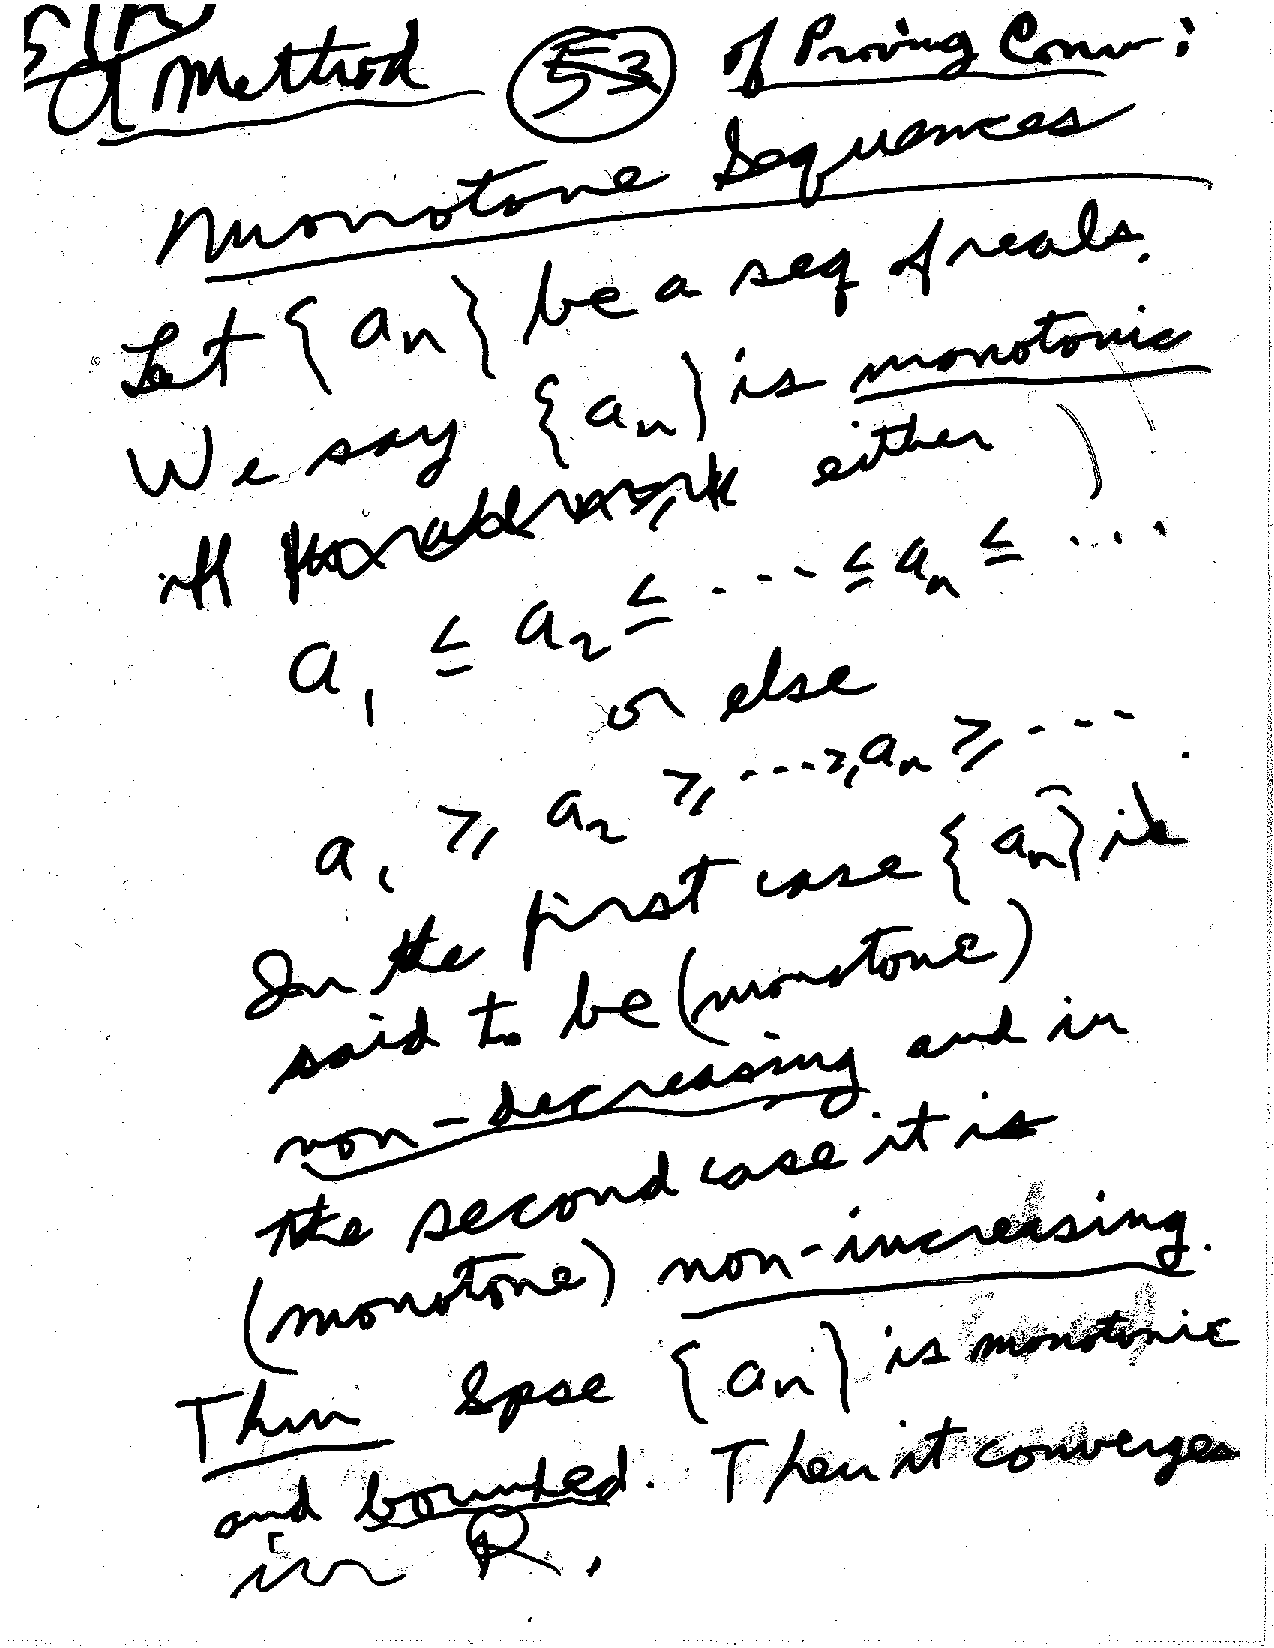
\includegraphics[scale=.5]{Pages/SL_8} 

\newpage
\underline{Theorem} Let $\{a_n\}$ be monotonic in R. Then in $R_\infty$\newline
$\lim_{n\rightarrow \infty}$ $a_n = 
\begin {cases}
sup $ $\{a_k\}$ $ & if a_1 \leq a_2 \leq a_3 \leq ...\\
inf $ $\{a_k\}$ $ & if a_1 \geq a_2 \geq ... 
\end {cases}$

\underline{Pf:} W l.o.g suppose $a_1 \leq a_2 \leq$ take away $b < suppose a_k$
Then $\exists k < \infty s.t. b < $ $\{a_k\}$. For all  $n \geq k, a_n \geq a_n so$
$a_n > b$. But also $a_n /leq suppose $ $\{a_k\}$

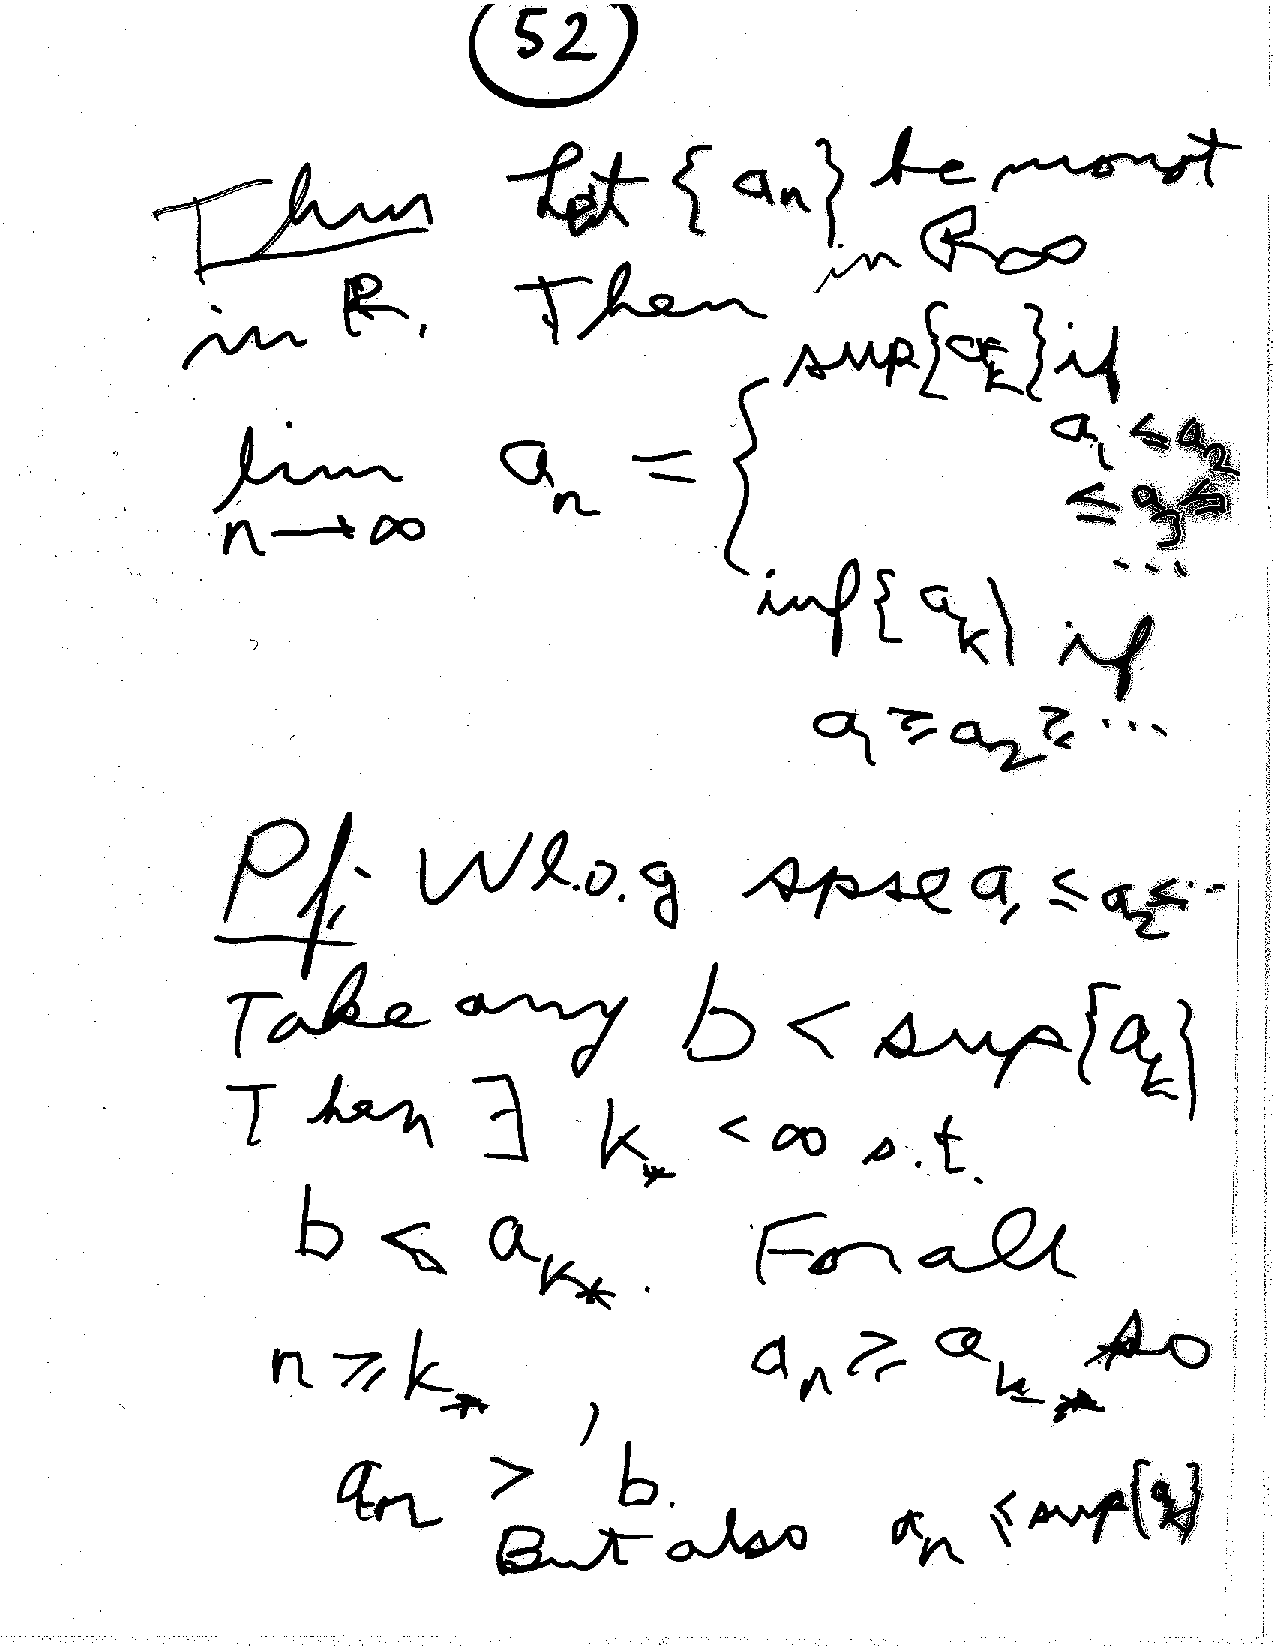
\includegraphics[scale=.5]{Pages/SL_9} 

\newpage

\underline{Theorem} Let $\{a_n\}$ be any sequence in $\mathbb{R}$ then $\exists 1 \leq n_1 < n_2 < ... s.t. a_{n_{1}}, a_{n_{2}},$ $a_{n_{3}}, ...$ is monotonic (i.e. $a_n$ has a monotonic sub sequence)\newline
\underline{Pf:} Either $a_1 \leq a_n$ for infinity many $n > 1$. Applying to each aj
Let J = $\{j\geq 1 : a_n \geq a_j$ for infinity many $n > j\}$
\underline{Cosel} $|J| = \infty $
Let $n_1$ = smallest $ j \in J$ $\exists n_2 > n_1$ with $n_2 /in J, ...$ ete get $ {n_k}$

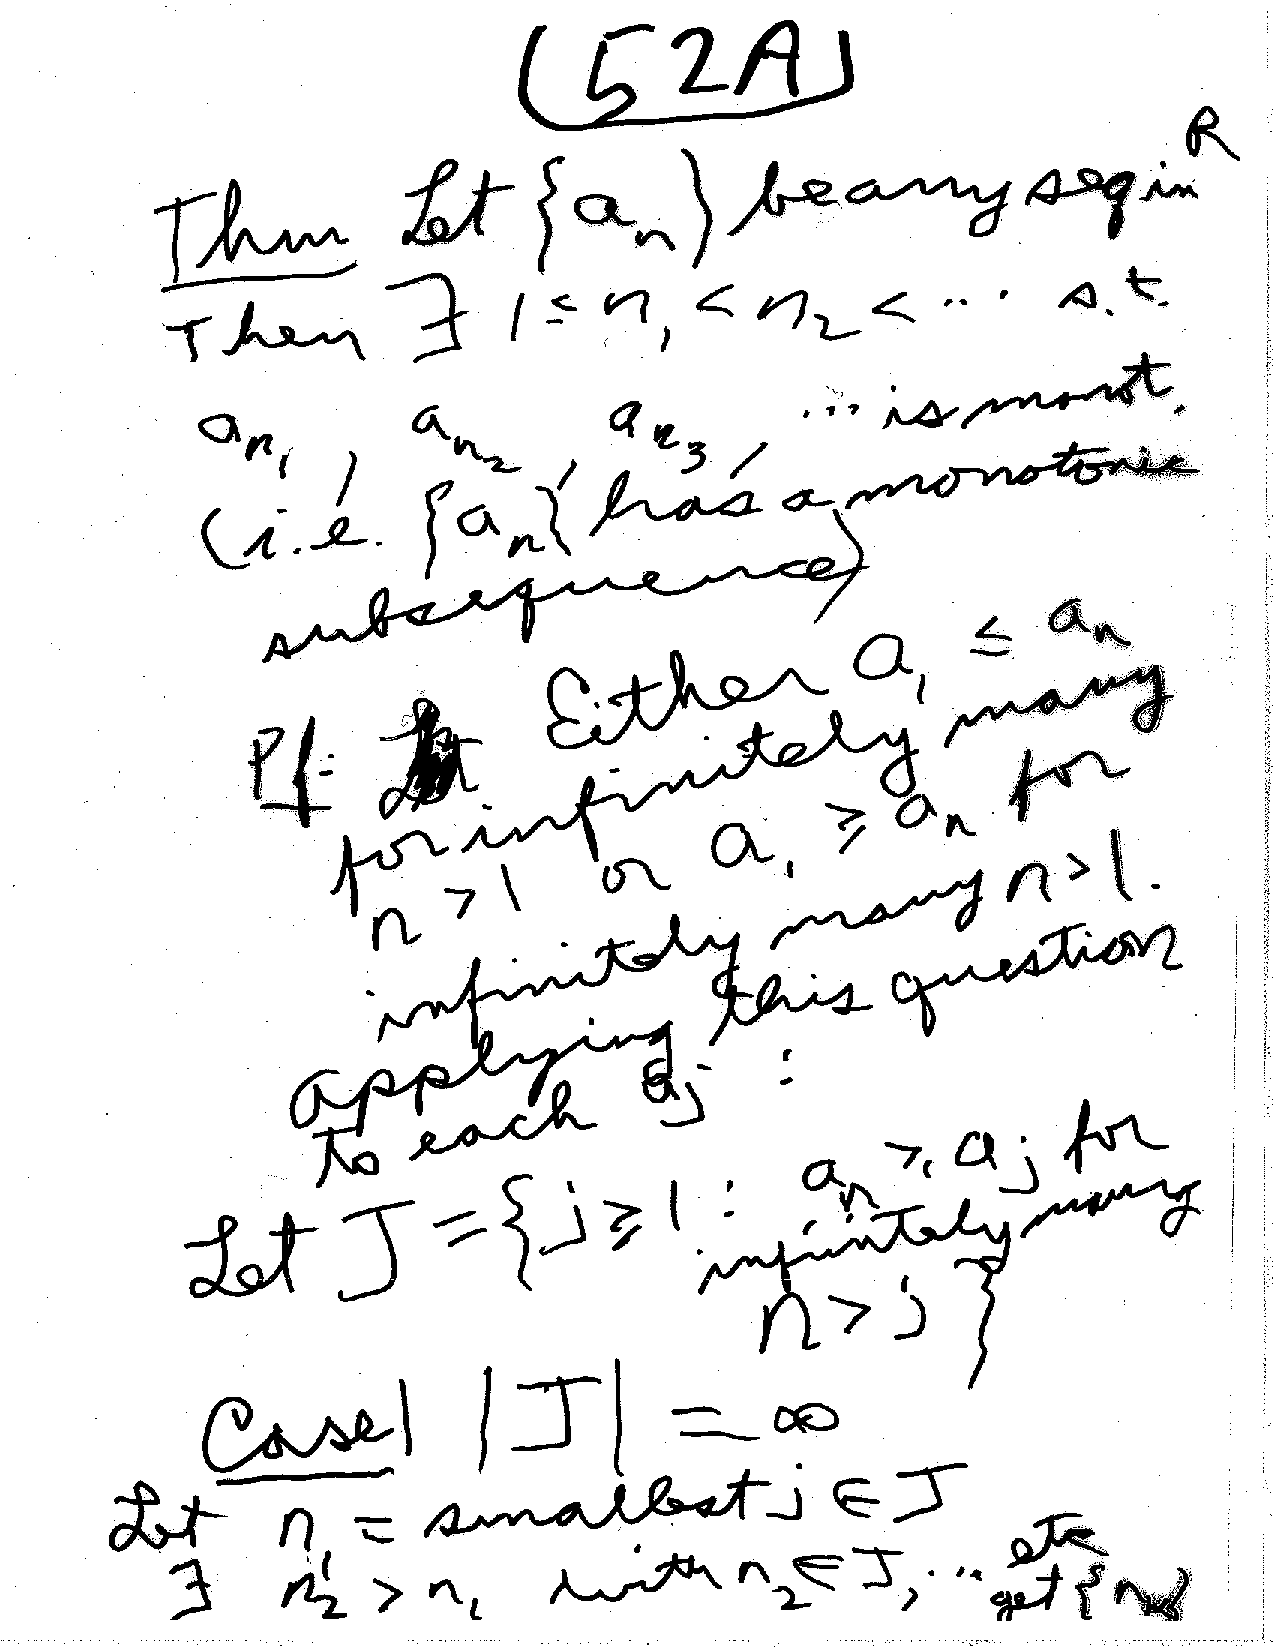
\includegraphics[scale=.5]{Pages/SL_10} 

\newpage

and $a_{n_{1}} \leq a_{n_{2}} \leq ...$ \newline
\underline{Case 2} $|J| < \infty$
take away $n_1 >$ one and max. $j \leftarrow J$ \newline
By construction, if $n_2$ is large enough $n_2 > n_1$ and $a_{n_{2}} < a_{n_{1}}$
By induction, having constructed $n_1 < n_2 < ... < n_k$ p.t. $a_{n_{1}} > a_{n_{2}} > ... > a_{n_{k}}$
$\exists n_{k+1} > n_k$ s.t. 
$a_{n_{k+1}} < a_{n_{k}}$ \newline
and so the theorem holds. 

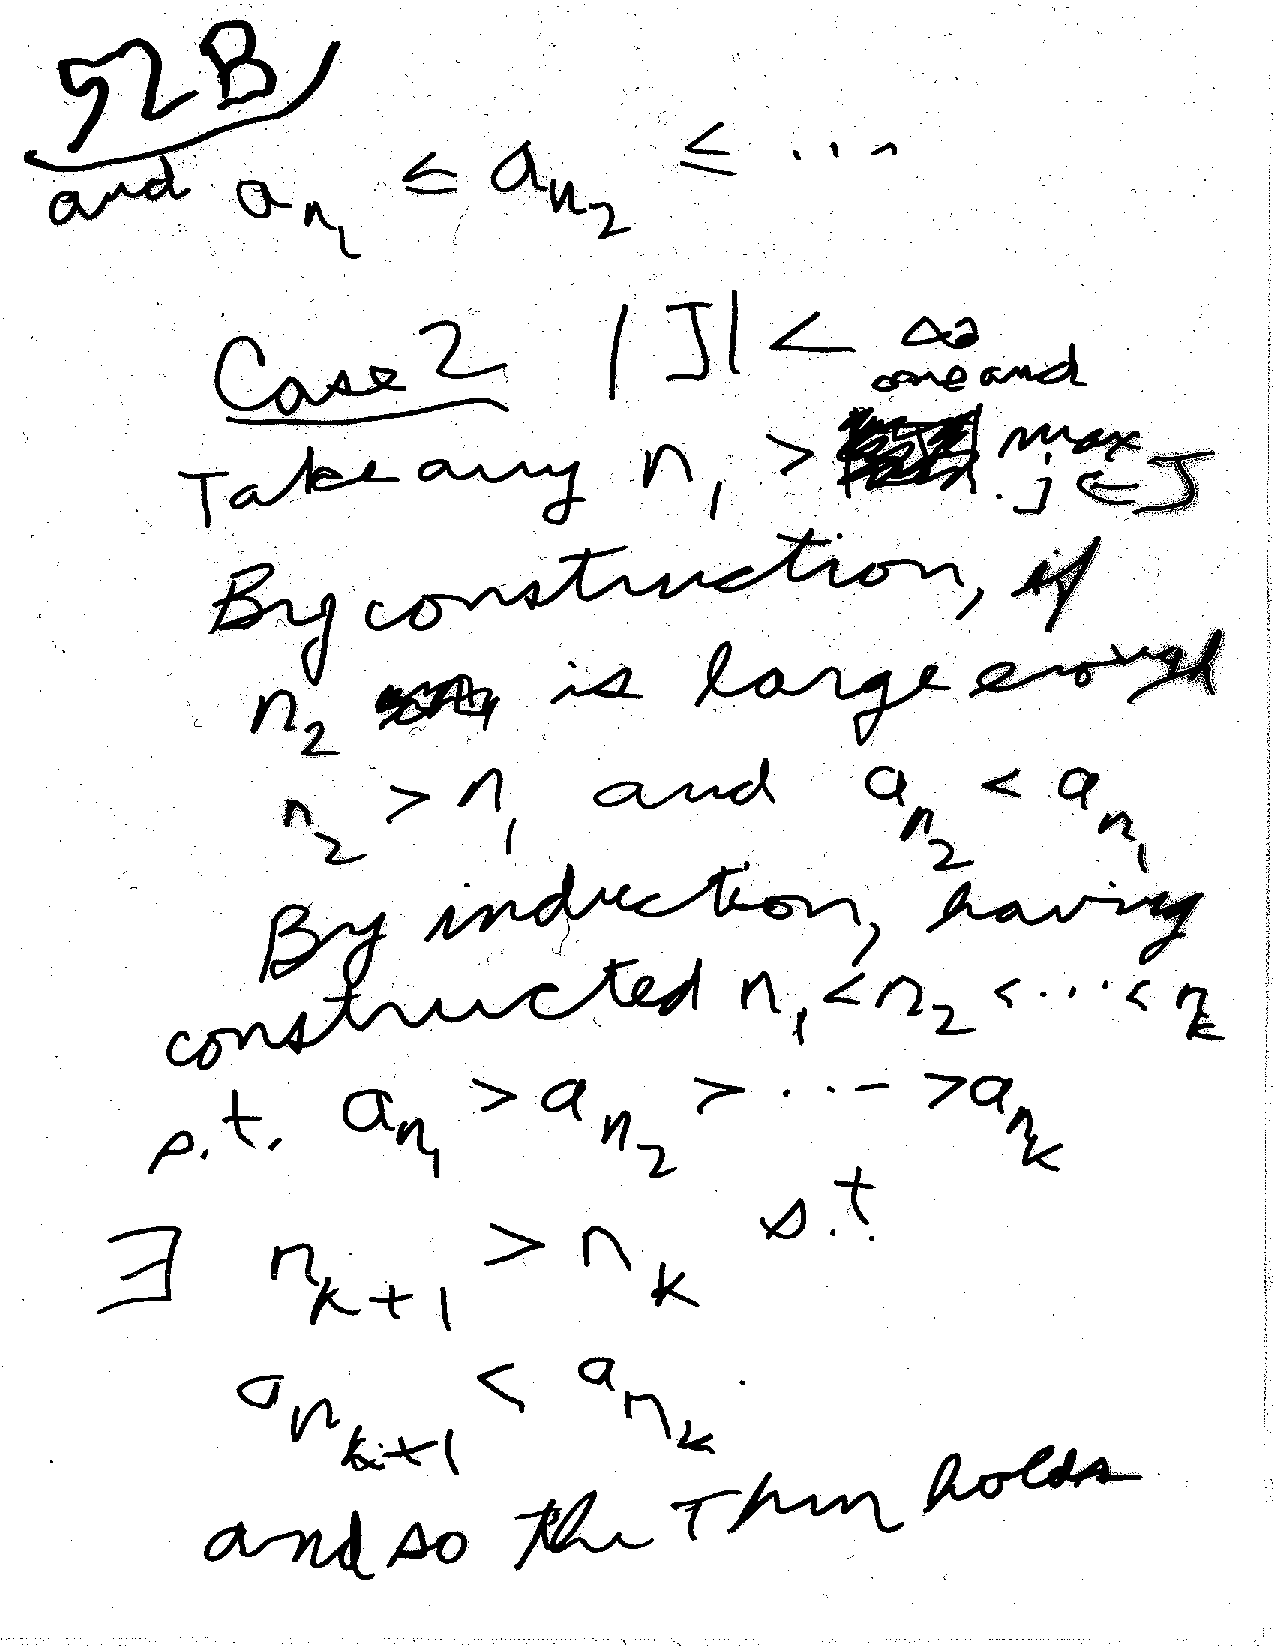
\includegraphics[scale=.5]{Pages/SL_11} 

\newpage
\section{Limit and Convergence}

%Joe: 50-51

%Quinten: 52-53

%Farishta: 53A-54A

\section{Infinite Series}

%Sukhreet: IS1 - IS 7

%Matthew: IS8 - IS15

%Will: IS16 - IS23

%Rebecca: IS24 - IS32

%Maady: IS33 - IS42

\section{Metric Spaces Part 1}

%Travis: M1 - M5

%Jerome: M6- M10



\section{Metric Spaces Part 2}


%Bryant: M1-M7

%Reshma: M8-M14

%Ethan: M15-M21





\end{document}